
\documentclass[letterpaper,hide notes,xcolor={table,svgnames},pdftex,10pt]{beamer}
\def\showexamples{t}


%\usepackage[svgnames]{xcolor}

%% Demo talk
%\documentclass[letterpaper,notes=show]{beamer}

\usecolortheme{crane}
\setbeamertemplate{navigation symbols}{}

\usetheme{MyPittsburgh}
%\usetheme{Frankfurt}

%\usepackage{tipa}

\usepackage{hyperref}
\usepackage{graphicx,xspace}
\usepackage[normalem]{ulem}
\usepackage{multicol}
\usepackage{amsmath,amssymb,amsthm,graphicx,xspace}
\newcommand\SF[1]{$\bigstar$\footnote{SF: #1}}

\usepackage[default]{sourcesanspro}
\usepackage[T1]{fontenc}
\usepackage[scaled]{beramono}
\usepackage{tikzpagenodes}

\newcounter{tmpnumSlide}
\newcounter{tmpnumNote}


% old question code
%\newcommand\question[1]{{$\bigstar$ \small \onlySlide{2}{#1}}}
% \newcommand\nquestion[1]{\ifdefined \presentationonly \textcircled{?} \fi \note{\par{\Large \textbf{?}} #1}}
% \newcommand\nanswer[1]{\note{\par{\Large \textbf{A}} #1}}


 \newcommand\mnote[1]{%
   \addtocounter{tmpnumSlide}{1}
   \ifdefined\showcues {~\tiny\fbox{\arabic{tmpnumSlide}}}\fi
   \note{\setlength{\parskip}{1ex}\addtocounter{tmpnumNote}{1}\textbf{\Large \arabic{tmpnumNote}:} {#1\par}}}

\newcommand\mmnote[1]{\note{\setlength{\parskip}{1ex}#1\par}}

%\newcommand\mnote[2][]{\ifdefined\handoutwithnotes {~\tiny\fbox{#1}}\fi
% \note{\setlength{\parskip}{1ex}\textbf{\Large #1:} #2\par}}

%\newcommand\mnote[2][]{{\tiny\fbox{#1}} \note{\setlength{\parskip}{1ex}\textbf{\Large #1:} #2\par}}

\newcommand\mquestion[2]{{~\color{red}\fbox{?}}\note{\setlength{\parskip}{1ex}\par{\Large \textbf{?}} #1} \note{\setlength{\parskip}{1ex}\par{\Large \textbf{A}} #2\par}\ifdefined \presentationonly \pause \fi}

\newcommand\blackboard[1]{%
\ifdefined   \showblackboard
  {#1}
  \else {\begin{center} \fbox{\colorbox{blue!30}{%
         \begin{minipage}{.95\linewidth}%
           \hspace{\stretch{1}} Some space intentionally left blank; done at the blackboard.%
         \end{minipage}}}\end{center}}%
         \fi%
}



%\newcommand\q{\tikz \node[thick,color=black,shape=circle]{?};}
%\newcommand\q{\ifdefined \presentationonly \textcircled{?} \fi}

\usepackage{listings}
\lstset{basicstyle=\footnotesize\ttfamily,
	breaklines=true,
	aboveskip=15pt,
  	belowskip=15pt,
	frame=lines,
	numbers=left, basicstyle=\scriptsize, numberstyle=\tiny, stepnumber=0, numbersep=2pt
}

\usepackage{siunitx}
\newcommand\sius[1]{\num[group-separator = {,}]{#1}\si{\micro\second}}
\newcommand\sims[1]{\num[group-separator = {,}]{#1}\si{\milli\second}}
\newcommand\sins[1]{\num[group-separator = {,}]{#1}\si{\nano\second}}
\sisetup{group-separator = {,}, group-digits = true}

%% -------------------- tikz --------------------
\usepackage{tikz}
\usetikzlibrary{positioning}
\usetikzlibrary{arrows,backgrounds,automata,decorations.shapes,decorations.pathmorphing,decorations.markings,decorations.text,decorations.pathreplacing}

\tikzstyle{place}=[circle,draw=blue!50,fill=blue!20,thick, inner sep=0pt,minimum size=6mm]
\tikzstyle{transition}=[rectangle,draw=black!50,fill=black!20,thick, inner sep=0pt,minimum size=4mm]

\tikzstyle{block}=[rectangle,draw=black, thick, inner sep=5pt]
\tikzstyle{bullet}=[circle,draw=black, fill=black, thin, inner sep=2pt]

\tikzstyle{pre}=[<-,shorten <=1pt,>=stealth',semithick]
\tikzstyle{post}=[->,shorten >=1pt,>=stealth',semithick]
\tikzstyle{bi}=[<->,shorten >=1pt,shorten <=1pt, >=stealth',semithick]

\tikzstyle{mut}=[-,>=stealth',semithick]

\tikzstyle{treereset}=[dashed,->, shorten >=1pt,>=stealth',thin]

\usepackage{ifmtarg}
\usepackage{xifthen}
\makeatletter
% new counter to now which frame it is within the sequence
\newcounter{multiframecounter}
% initialize buffer for previously used frame title
\gdef\lastframetitle{\textit{undefined}}
% new environment for a multi-frame
\newenvironment{multiframe}[1][]{%
\ifthenelse{\isempty{#1}}{%
% if no frame title was set via optional parameter,
% only increase sequence counter by 1
\addtocounter{multiframecounter}{1}%
}{%
% new frame title has been provided, thus
% reset sequence counter to 1 and buffer frame title for later use
\setcounter{multiframecounter}{1}%
\gdef\lastframetitle{#1}%
}%
% start conventional frame environment and
% automatically set frame title followed by sequence counter
\begin{frame}%
\frametitle{\lastframetitle~{\normalfont(\arabic{multiframecounter})}}%
}{%
\end{frame}%
}
\makeatother

\makeatletter
\newdimen\tu@tmpa%
\newdimen\ydiffl%
\newdimen\xdiffl%
\newcommand\ydiff[2]{%
    \coordinate (tmpnamea) at (#1);%
    \coordinate (tmpnameb) at (#2);%
    \pgfextracty{\tu@tmpa}{\pgfpointanchor{tmpnamea}{center}}%
    \pgfextracty{\ydiffl}{\pgfpointanchor{tmpnameb}{center}}%
    \advance\ydiffl by -\tu@tmpa%
}
\newcommand\xdiff[2]{%
    \coordinate (tmpnamea) at (#1);%
    \coordinate (tmpnameb) at (#2);%
    \pgfextractx{\tu@tmpa}{\pgfpointanchor{tmpnamea}{center}}%
    \pgfextractx{\xdiffl}{\pgfpointanchor{tmpnameb}{center}}%
    \advance\xdiffl by -\tu@tmpa%
}
\makeatother
\newcommand{\copyrightbox}[3][r]{%
\begin{tikzpicture}%
\node[inner sep=0pt,minimum size=2em](ciimage){#2};
\usefont{OT1}{phv}{n}{n}\fontsize{4}{4}\selectfont
\ydiff{ciimage.south}{ciimage.north}
\xdiff{ciimage.west}{ciimage.east}
\ifthenelse{\equal{#1}{r}}{%
\node[inner sep=0pt,right=1ex of ciimage.south east,anchor=north west,rotate=90]%
{\raggedleft\color{black!50}\parbox{\the\ydiffl}{\raggedright{}#3}};%
}{%
\ifthenelse{\equal{#1}{l}}{%
\node[inner sep=0pt,right=1ex of ciimage.south west,anchor=south west,rotate=90]%
{\raggedleft\color{black!50}\parbox{\the\ydiffl}{\raggedright{}#3}};%
}{%
\node[inner sep=0pt,below=1ex of ciimage.south west,anchor=north west]%
{\raggedleft\color{black!50}\parbox{\the\xdiffl}{\raggedright{}#3}};%
}
}
\end{tikzpicture}
}


%% --------------------

%\usepackage[excludeor]{everyhook}
%\PushPreHook{par}{\setbox0=\lastbox\llap{MUH}}\box0}

%\vspace*{\stretch{1}

%\setbox0=\lastbox \llap{\textbullet\enskip}\box0}

\setlength{\parskip}{\fill}

\newcommand\noskips{\setlength{\parskip}{1ex}}
\newcommand\doskips{\setlength{\parskip}{\fill}}

\newcommand\xx{\par\vspace*{\stretch{1}}\par}
\newcommand\xxs{\par\vspace*{2ex}\par}
\newcommand\tuple[1]{\langle #1 \rangle}
\newcommand\code[1]{{\sf \footnotesize #1}}
\newcommand\ex[1]{\uline{Example:} \ifdefined \presentationonly \pause \fi
  \ifdefined\showexamples#1\xspace\else{\uline{\hspace*{2cm}}}\fi}

\newcommand\ceil[1]{\lceil #1 \rceil}


\AtBeginSection[]
{
   \begin{frame}
       \frametitle{Outline}
       \tableofcontents[currentsection]
   \end{frame}
}



\pgfdeclarelayer{edgelayer}
\pgfdeclarelayer{nodelayer}
\pgfsetlayers{edgelayer,nodelayer,main}

\tikzstyle{none}=[inner sep=0pt]
\tikzstyle{rn}=[circle,fill=Red,draw=Black,line width=0.8 pt]
\tikzstyle{gn}=[circle,fill=Lime,draw=Black,line width=0.8 pt]
\tikzstyle{yn}=[circle,fill=Yellow,draw=Black,line width=0.8 pt]
\tikzstyle{empty}=[circle,fill=White,draw=Black]
\tikzstyle{bw} = [rectangle, draw, fill=blue!20, 
    text width=4em, text centered, rounded corners, minimum height=2em]
    
    \newcommand{\CcNote}[1]{% longname
	This work is licensed under the \textit{Creative Commons #1 3.0 License}.%
}
\newcommand{\CcImageBy}[1]{%
	\includegraphics[scale=#1]{creative_commons/cc_by_30.pdf}%
}
\newcommand{\CcImageSa}[1]{%
	\includegraphics[scale=#1]{creative_commons/cc_sa_30.pdf}%
}
\newcommand{\CcImageNc}[1]{%
	\includegraphics[scale=#1]{creative_commons/cc_nc_30.pdf}%
}
\newcommand{\CcGroupBySa}[2]{% zoom, gap
	\CcImageBy{#1}\hspace*{#2}\CcImageNc{#1}\hspace*{#2}\CcImageSa{#1}%
}
\newcommand{\CcLongnameByNcSa}{Attribution-NonCommercial-ShareAlike}

\newenvironment{changemargin}[1]{% 
  \begin{list}{}{% 
    \setlength{\topsep}{0pt}% 
    \setlength{\leftmargin}{#1}% 
    \setlength{\rightmargin}{1em}
    \setlength{\listparindent}{\parindent}% 
    \setlength{\itemindent}{\parindent}% 
    \setlength{\parsep}{\parskip}% 
  }% 
  \item[]}{\end{list}} 





\title{Lecture 20 --- Self-Optimizing Software }

\author{Jeff Zarnett \\ \small \texttt{jzarnett@uwaterloo.ca}}
\institute{Department of Electrical and Computer Engineering \\
  University of Waterloo}
\date{\today}


\begin{document}

\begin{frame}
  \titlepage

\end{frame}


\begin{frame}
\frametitle{Self-Optimizing Software}
The previous discussion was at compile-time... what about runtime?

The compiler can't help, but maybe a program can change itself to be better.

\begin{center}
	
\includegraphics[width=0.4\textwidth]{images/lawsoftime.png}
\end{center}

We'll start with the simple things and get more complex.
\end{frame}


\begin{frame}
\frametitle{Caching}

Your first thought about how a program might change itself for speed might be something like caching!

Keep track of the popular exchange rates?

If something becomes popular, it goes in the cache and becomes faster to access.

\end{frame}

\begin{frame}
\frametitle{Too Easy?}

You \textit{do} technically get different behaviour at runtime, but this is not quite what we wanted to talk about in this topic. 

\begin{center}
	
\includegraphics[width=0.3\textwidth]{images/caching.jpg}
\end{center}

It's too easy, and your program should probably be doing it already.

\end{frame}


\begin{frame}
\frametitle{Observe and Change}
Next idea:  your program's configuration changes at runtime to adapt to observed behaviour

This works becausse our initial guess might not be correct, but also because conditions can change at any time.

\end{frame}


\begin{frame}
\frametitle{Database Example}
Query processing: given a certain query, the database server comes up with an execution plan for how to carry it out.

A complex query may have multiple valid routes to executing it.

The server guesses what is correct, but may change its guess based on observation.

\end{frame}

\begin{frame}
\frametitle{Storage?}

Also, the server can update how it stores data based on how it's used.

Analogy: Excel sheet with student grades.

\begin{center}
	
\includegraphics[width=0.4\textwidth]{images/billgates.png}
\end{center}

This can apply to file storage on disk too.

\end{frame}


\begin{frame}
\frametitle{External Services}

There are three different servers where we can send messages and we'll measure and remember how long it took to get a response from that server. 
 
Geographically closest might be the fastest? Test this assumption!

\end{frame}

\begin{frame}
\frametitle{Genetic Algorithm}
If you've taken a course on algorithms, you might know this.

Inspired by natural selection.

\begin{center}
	
\includegraphics[width=0.4\textwidth]{images/genetic.jpg}
\end{center}

Create candidate solutions, evaluate for fitness, keep successful ones.

\end{frame}


\begin{frame}
\frametitle{If Applicable...}

This requires some parameters to configure, of course.

The problem also can't be pass/fail, but needs to have degrees of success.

The fitness function might find a local maximum rather than a global one.

Finding the solution might be fairly slow.

\end{frame}


\begin{frame}
\frametitle{Genetic Algorithms Do What?}

How does it help? Optimize our configuration parameters.

Recall our earlier discussion of Google Maps: decision based on parameters.

\begin{itemize}
	\item Number of routes to evaluate
	\item Heuristic for generating routes to evaluate
	\item Decay of traffic information reported by other motorists
	\item Time of day and month and if it's a holiday
	\item Search radius for alternate routes
\end{itemize}

\end{frame}


\begin{frame}
\frametitle{Does Google Maps Work Like This?}

This isn't necessarily how Google does it.

Choosing correct parameters by hand is very difficult.

The problem is likely non-linear.

\end{frame}


\begin{frame}
\frametitle{Hotspot Compiler}

Some compiler optimizations are always a clear win; others only sometimes.

Inlining is sometimes good, but can make things worse. 

Compile-time decisions usually are permanent, but there's also the JVM...

\begin{center}
	
\includegraphics[width=0.4\textwidth]{images/problemfactory.jpg}
\end{center}

\end{frame}


\begin{frame}
\frametitle{Java Can Be Good?}

There's the JIT (Just-in-Time) compiler; so decisions can be made at runtime what to compiler.

The runtime can observe the actual runtime behaviour and change what decision it makes.

That's more helpful in some scenarios (inlining) than others (branch prediction).

\end{frame}

\begin{frame}
\frametitle{Bonus Features}
Some other things that can happen at runtime worth talking about:

\begin{itemize}
	\item Escape Analysis
	\item On-Stack Replacement
	\item Intrinsics
\end{itemize}

\end{frame}


\begin{frame}
\frametitle{Escape Analysis}

``Are there any side effects visible outside a method?''

\begin{center}
	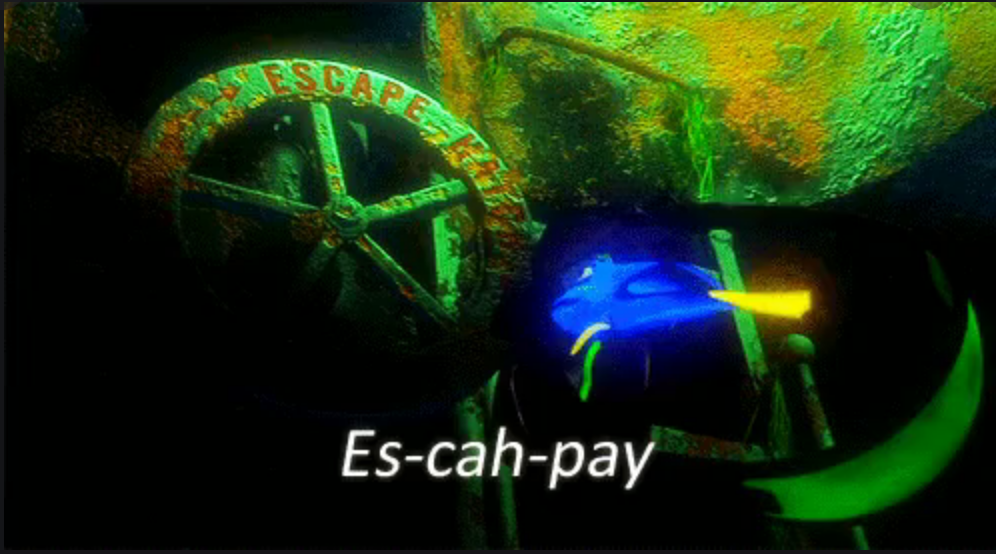
\includegraphics[width=0.3\textwidth]{images/escape.png}
\end{center}

If no, we can skip some heap allocation and maybe change the scope of locks.

Lock elision: don't use a lock if there's no need for one.

Lock coarsening: make critical sections bigger; reduce lock/unlock events.

\end{frame}


\begin{frame}
\frametitle{On-Stack Replacement}

``I know a shortcut.''

The VM can switch between different implementations of the same method.

If a function is \alert{hot}, use a more optimized version.

There's a cost to swapping in the stack frame, but long-term savings.

\end{frame}

\begin{frame}
\frametitle{Ever Debugged in Java/Kotlin?}

When you have the debugger attached you can swap in frames with new code.

Very helpful when it takes a lot of work to reproduce a problem...\\
\quad Or the app takes a long time to start.

\end{frame}


\begin{frame}
\frametitle{Intrinsics}

``Prepare in advance the best version for this architecture.''

There are precompiled segments for specific platforms like x86.

Originally in \CPP but now you can convert Java bye code directly. 

Intrinsics are complicated... But closest to what you maybe imagined.

\end{frame}


\begin{frame}
\frametitle{Rust and the Hotspot}

Rust doesn't have a runtime as a design choice.

Decisions made at compile-time will stand... Unless...

\begin{center}
	
\includegraphics[width=0.5\textwidth]{images/bigbrain.jpg}
\end{center}

\end{frame}


\begin{frame}
\frametitle{Precompiled}

One possibility is to have different versions of the code compiled and swap them in as needed.

Of course we have to prepare them all and it increases compile time.

We're still guessing what we think, but we get more than one guess!

Swapping it in at runtime requires some coordination.

But why not if-statements?

\end{frame}

\begin{frame}
\frametitle{Code Generation}

So, you want to compile some code. 

Don't write a compiler... Use the one on the current system!

Requiring a specific compiler might be limiting in deployment.

\end{frame}


\begin{frame}
\frametitle{We're In Business}

First, take the binary code of the segment that we want to optimize and then have the compiler take a look at it. 

The compiler will then take the binary, convert it to its internal representation (the intermediate representation), then optimize it, and compile it. 

The new binary code can get swapped in when it's ready.

\end{frame}

\begin{frame}
\frametitle{Does it Work?}


Does this work? Yes!

A calculation on a matrix of size 649 $\times$ 649 for 20~000 iterations. 

Here's a graph of the performance results from the improved code:

\begin{center}
	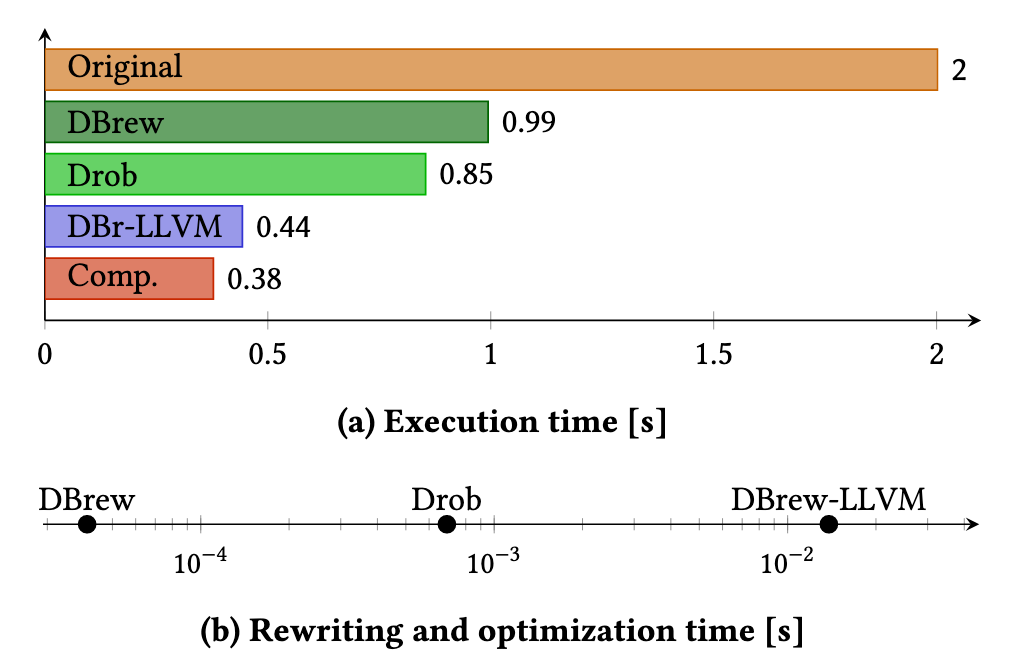
\includegraphics[width=0.6\textwidth]{images/rewriting.png}
\end{center}

Given the right workload, this is worth doing!

\end{frame}


\begin{frame}
\frametitle{Unfortunately...}

\begin{center}
	
\includegraphics[width=0.45\textwidth]{images/amongus.png}
\end{center}

``Program sus.''

\end{frame}

\begin{frame}
\frametitle{The Arms Race Continues}


Programs that rewrite themselves are frequently judged as suspicious by anti-virus and anti-malware software. 

This is part of the arms race between anti-virus software and software.

Anti-malware software end-users have installed may affect the experience.

\end{frame}


\end{document}

